\documentclass[border=0bp]{standalone}
\usepackage[T1]{fontenc}
\usepackage{times,amsmath,amssymb,graphicx,xcolor}
\usepackage{tikz}
\usetikzlibrary{arrows.meta,calc,positioning,patterns}
\pdfinfoomitdate=1
\pdftrailerid{}
\definecolor{ink}{HTML}{202020}
\definecolor{muted}{HTML}{626262}
\definecolor{hairline}{HTML}{B9B9B9}
\definecolor{accent}{HTML}{284E67}
\definecolor{signal}{HTML}{A33D36}
\definecolor{objectred}{HTML}{D45B59}
\definecolor{objectgreen}{HTML}{55A870}
\definecolor{objectblue}{HTML}{507BC2}
\definecolor{teal}{HTML}{087E81}
\definecolor{ochre}{HTML}{B27A46}
\definecolor{violet}{HTML}{7563A6}
\tikzset{
 every node/.style={font=\fontsize{10.5}{12.5}\selectfont,inner sep=0bp,outer sep=0bp,text=ink},
 flow/.style={draw=ink,line width=.45bp,-{Latex[length=3bp,width=2bp]}},
 auxflow/.style={draw=muted,line width=.35bp,-{Latex[length=3bp,width=2bp]}},
 measure/.style={draw=ink,line width=.4bp,{Latex[length=2.4bp,width=1.6bp]}-{Latex[length=2.4bp,width=1.6bp]}},
 envelope/.style={draw=muted,line width=.35bp,dash pattern=on 2bp off 1.5bp,fill=none},
 frame/.style={draw=hairline,line width=.35bp,fill=none},
 leader/.style={draw=muted,line width=.35bp},
 module/.style={draw=ink,line width=.45bp,fill=white,minimum height=30bp,align=center,inner xsep=3bp,inner ysep=3bp},
}
\begin{document}
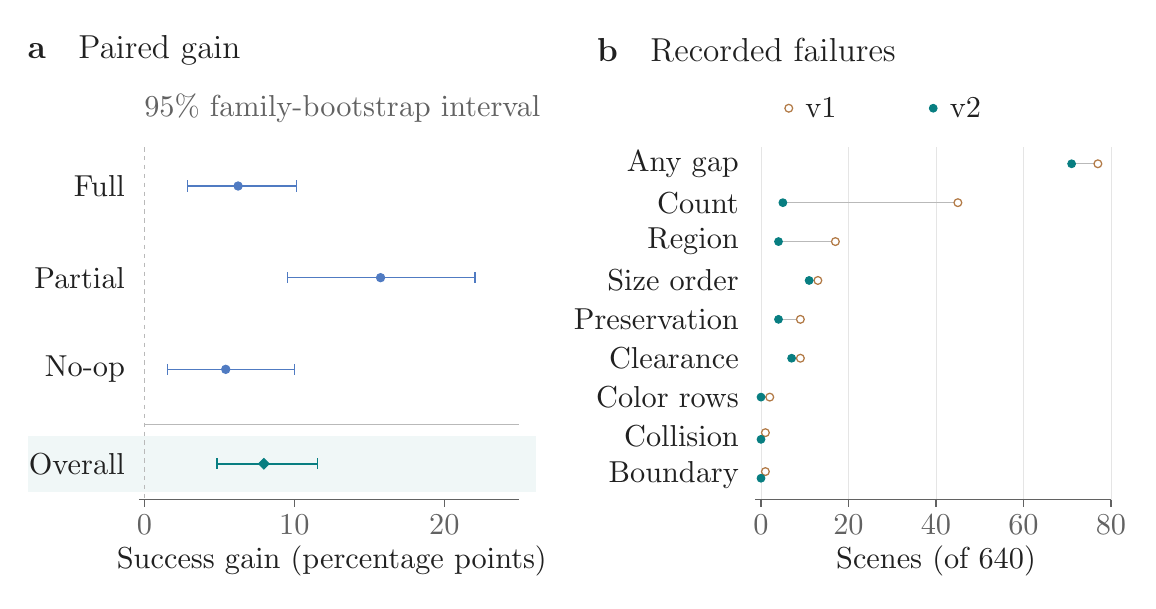
\begin{tikzpicture}[x=1bp,y=-1bp,line cap=butt,line join=miter]
\node[anchor=west,text=ink,font=\fontsize{11.5}{13.0}\selectfont] at (0.00000,8.00000) {\textbf{a}\quad Paired gain};
\node[anchor=west,text=ink,font=\fontsize{11.5}{13.0}\selectfont] at (205.00000,8.00000) {\textbf{b}\quad Recorded failures};
\begin{scope}[shift={(0,4)}]
\node[anchor=west,text=muted,font=\fontsize{10.5}{12.0}\selectfont] at (42.00000,25.00000) {95\% family-bootstrap interval};
\path[draw=ochre,fill=white,line width=.45bp] (274.00000,25.00000) circle[radius=1.4bp];
\node[anchor=west,text=ink,font=\fontsize{10.5}{12.0}\selectfont] at (280.00000,25.00000) {v1};
\path[draw=teal,fill=teal,line width=.35bp] (326.00000,25.00000) circle[radius=1.4bp];
\node[anchor=west,text=ink,font=\fontsize{10.5}{12.0}\selectfont] at (332.00000,25.00000) {v2};
\path[fill=teal!6,draw=none] (0,143) rectangle (183,163);
\draw[draw=hairline,line width=.35bp,dash pattern=on 1.6bp off 1.6bp] (42.00000,39.00000) -- (42.00000,166.00000);
\draw[draw=hairline,line width=.3bp] (42.00000,139.00000) -- (177.00000,139.00000);
\draw[draw=black!10,line width=.3bp] (264.00000,39.00000) -- (264.00000,166.00000);
\draw[draw=black!10,line width=.3bp] (295.50000,39.00000) -- (295.50000,166.00000);
\draw[draw=black!10,line width=.3bp] (327.00000,39.00000) -- (327.00000,166.00000);
\draw[draw=black!10,line width=.3bp] (358.50000,39.00000) -- (358.50000,166.00000);
\draw[draw=black!10,line width=.3bp] (390.00000,39.00000) -- (390.00000,166.00000);
\draw[draw=muted,line width=.4bp] (40.00000,166.00000) -- (177.00000,166.00000);
\draw[draw=muted,line width=.4bp] (42.00000,166.00000) -- (42.00000,168.50000);
\node[anchor=center,text=muted,font=\fontsize{10.5}{12.0}\selectfont] at (42.00000,175.00000) {0};
\draw[draw=muted,line width=.4bp] (96.00000,166.00000) -- (96.00000,168.50000);
\node[anchor=center,text=muted,font=\fontsize{10.5}{12.0}\selectfont] at (96.00000,175.00000) {10};
\draw[draw=muted,line width=.4bp] (150.00000,166.00000) -- (150.00000,168.50000);
\node[anchor=center,text=muted,font=\fontsize{10.5}{12.0}\selectfont] at (150.00000,175.00000) {20};
\draw[draw=muted,line width=.4bp] (262.00000,166.00000) -- (390.00000,166.00000);
\draw[draw=muted,line width=.4bp] (264.00000,166.00000) -- (264.00000,168.50000);
\node[anchor=center,text=muted,font=\fontsize{10.5}{12.0}\selectfont] at (264.00000,175.00000) {0};
\draw[draw=muted,line width=.4bp] (295.50000,166.00000) -- (295.50000,168.50000);
\node[anchor=center,text=muted,font=\fontsize{10.5}{12.0}\selectfont] at (295.50000,175.00000) {20};
\draw[draw=muted,line width=.4bp] (327.00000,166.00000) -- (327.00000,168.50000);
\node[anchor=center,text=muted,font=\fontsize{10.5}{12.0}\selectfont] at (327.00000,175.00000) {40};
\draw[draw=muted,line width=.4bp] (358.50000,166.00000) -- (358.50000,168.50000);
\node[anchor=center,text=muted,font=\fontsize{10.5}{12.0}\selectfont] at (358.50000,175.00000) {60};
\draw[draw=muted,line width=.4bp] (390.00000,166.00000) -- (390.00000,168.50000);
\node[anchor=center,text=muted,font=\fontsize{10.5}{12.0}\selectfont] at (390.00000,175.00000) {80};
\node[anchor=east,text=ink,font=\fontsize{10.5}{12.0}\selectfont] at (35.00000,53.00000) {Full};
\draw[draw=objectblue,line width=.55bp] (57.46875,53.00000) -- (96.84375,53.00000);
\draw[draw=objectblue,line width=.4bp] (57.46875,51.00000) -- (57.46875,55.00000);
\draw[draw=objectblue,line width=.4bp] (96.84375,51.00000) -- (96.84375,55.00000);
\path[draw=objectblue,fill=objectblue,line width=.35bp] (75.75000,53.00000) circle[radius=1.5bp];
\node[anchor=east,text=ink,font=\fontsize{10.5}{12.0}\selectfont] at (35.00000,86.00000) {Partial};
\draw[draw=objectblue,line width=.55bp] (93.42857,86.00000) -- (161.05512,86.00000);
\draw[draw=objectblue,line width=.4bp] (93.42857,84.00000) -- (93.42857,88.00000);
\draw[draw=objectblue,line width=.4bp] (161.05512,84.00000) -- (161.05512,88.00000);
\path[draw=objectblue,fill=objectblue,line width=.35bp] (127.03937,86.00000) circle[radius=1.5bp];
\node[anchor=east,text=ink,font=\fontsize{10.5}{12.0}\selectfont] at (35.00000,119.00000) {No-op};
\draw[draw=objectblue,line width=.55bp] (50.43750,119.00000) -- (96.00000,119.00000);
\draw[draw=objectblue,line width=.4bp] (50.43750,117.00000) -- (50.43750,121.00000);
\draw[draw=objectblue,line width=.4bp] (96.00000,117.00000) -- (96.00000,121.00000);
\path[draw=objectblue,fill=objectblue,line width=.35bp] (71.30233,119.00000) circle[radius=1.5bp];
\node[anchor=east,text=ink,font=\fontsize{10.5}{12.0}\selectfont] at (35.00000,153.00000) {Overall};
\draw[draw=teal,line width=.55bp] (68.15625,153.00000) -- (104.43750,153.00000);
\draw[draw=teal,line width=.4bp] (68.15625,151.00000) -- (68.15625,155.00000);
\draw[draw=teal,line width=.4bp] (104.43750,151.00000) -- (104.43750,155.00000);
\path[draw=teal,fill=teal,line width=.35bp] (85.03125,151.10000) -- (86.93125,153.00000) -- (85.03125,154.90000) -- (83.13125,153.00000) -- cycle;
\node[anchor=east,text=ink,font=\fontsize{10.5}{12.0}\selectfont] at (256.00000,45.00000) {Any gap};
\draw[draw=hairline,line width=.5bp] (385.27500,45.00000) -- (375.82500,45.00000);
\path[draw=ochre,fill=white,line width=.45bp] (385.27500,45.00000) circle[radius=1.4bp];
\path[draw=teal,fill=teal,line width=.35bp] (375.82500,45.00000) circle[radius=1.4bp];
\node[anchor=east,text=ink,font=\fontsize{10.5}{12.0}\selectfont] at (256.00000,59.00000) {Count};
\draw[draw=hairline,line width=.5bp] (334.87500,59.00000) -- (271.87500,59.00000);
\path[draw=ochre,fill=white,line width=.45bp] (334.87500,59.00000) circle[radius=1.4bp];
\path[draw=teal,fill=teal,line width=.35bp] (271.87500,59.00000) circle[radius=1.4bp];
\node[anchor=east,text=ink,font=\fontsize{10.5}{12.0}\selectfont] at (256.00000,73.00000) {Region};
\draw[draw=hairline,line width=.5bp] (290.77500,73.00000) -- (270.30000,73.00000);
\path[draw=ochre,fill=white,line width=.45bp] (290.77500,73.00000) circle[radius=1.4bp];
\path[draw=teal,fill=teal,line width=.35bp] (270.30000,73.00000) circle[radius=1.4bp];
\node[anchor=east,text=ink,font=\fontsize{10.5}{12.0}\selectfont] at (256.00000,87.00000) {Size order};
\draw[draw=hairline,line width=.5bp] (284.47500,87.00000) -- (281.32500,87.00000);
\path[draw=ochre,fill=white,line width=.45bp] (284.47500,87.00000) circle[radius=1.4bp];
\path[draw=teal,fill=teal,line width=.35bp] (281.32500,87.00000) circle[radius=1.4bp];
\node[anchor=east,text=ink,font=\fontsize{10.5}{12.0}\selectfont] at (256.00000,101.00000) {Preservation};
\draw[draw=hairline,line width=.5bp] (278.17500,101.00000) -- (270.30000,101.00000);
\path[draw=ochre,fill=white,line width=.45bp] (278.17500,101.00000) circle[radius=1.4bp];
\path[draw=teal,fill=teal,line width=.35bp] (270.30000,101.00000) circle[radius=1.4bp];
\node[anchor=east,text=ink,font=\fontsize{10.5}{12.0}\selectfont] at (256.00000,115.00000) {Clearance};
\draw[draw=hairline,line width=.5bp] (278.17500,115.00000) -- (275.02500,115.00000);
\path[draw=ochre,fill=white,line width=.45bp] (278.17500,115.00000) circle[radius=1.4bp];
\path[draw=teal,fill=teal,line width=.35bp] (275.02500,115.00000) circle[radius=1.4bp];
\node[anchor=east,text=ink,font=\fontsize{10.5}{12.0}\selectfont] at (256.00000,129.00000) {Color rows};
\draw[draw=hairline,line width=.5bp] (267.15000,129.00000) -- (264.00000,129.00000);
\path[draw=ochre,fill=white,line width=.45bp] (267.15000,129.00000) circle[radius=1.4bp];
\path[draw=teal,fill=teal,line width=.35bp] (264.00000,129.00000) circle[radius=1.4bp];
\node[anchor=east,text=ink,font=\fontsize{10.5}{12.0}\selectfont] at (256.00000,143.00000) {Collision};
\draw[draw=hairline,line width=.5bp] (265.57500,141.80000) -- (264.00000,144.20000);
\path[draw=ochre,fill=white,line width=.45bp] (265.57500,141.80000) circle[radius=1.4bp];
\path[draw=teal,fill=teal,line width=.35bp] (264.00000,144.20000) circle[radius=1.4bp];
\node[anchor=east,text=ink,font=\fontsize{10.5}{12.0}\selectfont] at (256.00000,157.00000) {Boundary};
\draw[draw=hairline,line width=.5bp] (265.57500,155.80000) -- (264.00000,158.20000);
\path[draw=ochre,fill=white,line width=.45bp] (265.57500,155.80000) circle[radius=1.4bp];
\path[draw=teal,fill=teal,line width=.35bp] (264.00000,158.20000) circle[radius=1.4bp];
\node[anchor=center,text=ink,font=\fontsize{10.5}{12.0}\selectfont] at (109.50000,188.00000) {Success gain (percentage points)};
\node[anchor=center,text=ink,font=\fontsize{10.5}{12.0}\selectfont] at (327.00000,188.00000) {Scenes (of 640)};
\end{scope}

\pgfresetboundingbox
\path[use as bounding box] (0,0) rectangle (396,199);
\end{tikzpicture}
\end{document}
